\documentclass[12pt, titlepage]{article}

\usepackage[utf8]{inputenc}
\usepackage[spanish]{babel}
\usepackage{hyperref}
\hypersetup{
    colorlinks,
    linkcolor = blue
}
\usepackage{titlesec}
\newcommand{\sectionbreak}{\clearpage}
\usepackage{amsmath,amsfonts,mathtools,amssymb,physics}
\usepackage{tikz,pgf,pgfplots,listings,xcolor,framed,booktabs,longtable}
\usepackage[autostyle]{csquotes}
\usetikzlibrary{external,arrows}
\tikzexternalize[prefix=figures/]
%\pgfplotsset{compat=1.11}

\definecolor{codegreen}{rgb}{0,0.6,0}
\definecolor{codegray}{rgb}{0.5,0.5,0.5}
\definecolor{codepurple}{rgb}{0.58,0,0.82}
\definecolor{backcolour}{rgb}{0.95,0.95,0.92}

\lstdefinestyle{mystyle}{
    backgroundcolor=\color{backcolour},
    commentstyle=\color{codegreen},
    keywordstyle=\color{magenta},
    numberstyle=\tiny\color{codegray},
    stringstyle=\color{codepurple},
    basicstyle=\footnotesize,
    breakatwhitespace=false,
    breaklines=true,
    captionpos=b,
    keepspaces=true,
    numbers=none,
    numbersep=5pt,
    showspaces=false,
    showstringspaces=false,
    showtabs=false,
    tabsize=2
}

\lstdefinelanguage{PDDL}
{
  sensitive=false,    % not case-sensitive
  morecomment=[l]{;}, % line comment
  alsoletter={:,-},   % consider extra characters
  morekeywords={
    define,domain,problem,not,and,or,when,forall,exists,either,
    :domain,:requirements,:types,:objects,:constants,
    :predicates,:action,:parameters,:precondition,:effect,
    :fluents,:primary-effect,:side-effect,:init,:goal,
    :strips,:adl,:equality,:typing,:conditional-effects,
    :negative-preconditions,:disjunctive-preconditions,
    :existential-preconditions,:universal-preconditions,:quantified-preconditions,
    :functions,assign,increase,decrease,scale-up,scale-down,
    :metric,minimize,maximize,
    :durative-actions,:duration-inequalities,:continuous-effects,
    :durative-action,:duration,:condition,
  }
}

\lstset{style=mystyle,basicstyle=\ttfamily}

\newcommand*\dif{\mathop{}\!\mathrm{d}}

%\usepackage[margin=1in,a4paper]{geometry}
\usepackage{parskip}

\begin{document}

\begin{titlepage}
    \centering
    \vspace{0.5 cm}
    \begin{center}
        \textsc{\Large Universitat Politècnica de Catalunya}\\[2.0 cm]
    \end{center}% University Name
    \textsc{\Large Laboratorio de Inteligencia Artificial }\\[0.5 cm]
    \rule{\linewidth}{0.2 mm} \\[0.4 cm]
    { \huge \bfseries Práctica de planificación}\\
    \rule{\linewidth}{0.2 mm} \\[1.5 cm]
    
    \vfill

    \begin{minipage}{\textwidth}

        \begin{flushright} \large
            \emph{Realizado por :} \\
            Muntaner, Joan \\
            Lanchares, Ernesto \\
            López, Ferran \\
            Zhang, Niebo
        \end{flushright}

    \end{minipage}\\[2 cm]

    
\includegraphics[scale = 0.3]{UPCLogo.png}
    \vspace{0.5cm}
\end{titlepage}

\tableofcontents

\section{Modelado del dominio}
\subsection{Tipos y funciones}

Para modelar el problema, hemos empleado solamente dos tipos: Tarea y
Programador. Hemos decidido no usar el tipo Revisión ya que a
nuestro parecer tan solo complicaba el código.

\subsubsection{Tarea}
Dentro de nuestro dominio existen Tareas, cada Tarea tiene asociada una
dificultad y unas horas. Para representarlo en nuestro dominio, hemos creado dos
funciones
\begin{lstlisting}[language=PDDL]
    (dificultad ?t - Tarea)
    (horas ?t - Tarea)
\end{lstlisting}
que serán constantes y las definiremos para el problema concreto.

\subsubsection{Programador}
Dentro de nuestro dominio, también existen Programadores. Cada Programador tien
asociada una habilidad y una calidad. Estas características las representaremos
por dos funciones
\begin{lstlisting}[language=PDDL]
    (habilidad ?p - Programador)
    (calidad ?p - Programador)
\end{lstlisting}
que serán constantes y las inicializaremos en el problema.

Además, a partir de la extensión 3, se requiere que el número de programas
asociados a cada programador sea como mucho 2. Para implementar esta
funcionalidad hemos creado la función
\begin{lstlisting}[language=PDDL]
    (tareas-asignadas ?p - Programador)
\end{lstlisting}
que inicializaremos a cero en el problema e iremos aumentando a medida que
vayamos asignando tareas a cada programador.

\subsection{Fluentes}

Notemos que los fluentes tan solo los utilizamos a partir de la extensión 2,
que es donde se requieren. Nosotros hemos definido dos fluentes, ambos los
definiremos a cero en el programa.

\subsubsection{Fluente \texttt{total}}
Este fluente indica el número total de horas invertidas en realizar o revisar
las tareas y lo incrementaremos (en la cantidad correspondiente) cada vez que
asignemos realizar o revisar una tarea a un programador.

\subsubsection{Fluente \texttt{num-persnas}}
Este fluente indica el número total de personas que realizan tareas (no contamos
la revisión). Cada vez que asignamos una tarea a alguien incrementaremos
\texttt{num-personas} si esa persona no tenia nunguna tarea asiganada antes y la
mantendremos igual si la persona ya tenía una tarea asignada.

\subsection{Predicados}
En nuestra representación del dominio, utilizaremos tres predicados:
\begin{lstlisting}[language=PDDL]
    (realizada ?t - Tarea)
    (trabaja ?p - Programador ?t - Tarea)
    (revisada ?t - Tarea)
\end{lstlisting}

\texttt{realizada} significa que la tarea en cuestión ya ha sido realizada,
\texttt{revisada} significa que la tarea en cuestión ya ha sido revisada y
\texttt{trabaja} significa que el programador en cuestión es el encargado de
realizar la tarea.

Notamos que el predicado \texttt{realizada} no es necesario, porque existe la
equivalencia
\[
    \texttt{realizadada}(t) \iff \exists p \in \texttt{Programadores} \text{ tal
    que} \texttt{trabaja}(p, t)
\]
que podemos traducir a PDDL como
\begin{lstlisting}[escapeinside={(*}{*)},language=PDDL]
(realizada ?t) (*$\iff$*) (exists (?p - Programador) (trabaja ?p ?t))
\end{lstlisting}

Es decir, que podriamos eliminar un predicado si lo sustituimos por esa
expresión. Sin embargo, en las pruebas realizadas nos hemos encontrado que
realizar este cambio supone un incremento sustancial de tiempo y por lo tanto no merece la pena.

\subsection{Acciones}
En nuestro dominio, contamos con dos acciones: la acción de realizar una tarea a
un programador y la acción de revisar una tarea.

\subsubsection{Realizar}
A la hora de asignar tareas a programadores tenemos en cuenta diversos factores,
que se traducen a precondiciones. Las precondiciones son
\begin{itemize}
    \item La tarea no está realizada ya.
    \item El programador tiene habilidad suficiente para realizar la tarea.
    \item (Solo a partir de la extensión 3) El programador ha realizado menos de
        dos tareas previamente.
\end{itemize}

Y como consecuencias tendrá
\begin{itemize}
    \item la tarea pasa a estar realizada.
\end{itemize}
A partir de la extensión 1
\begin{itemize}
    \item La tarea no está revisada.
    \item La tarea ha sido realizada por el programador en cuestión.
\end{itemize}
A partir de la extensión 2
\begin{itemize}
    \item El número total de horas aumenta en el número de horas de la tarea.
    \item El número total de horas aumenta en 2 si la dificultad de la tarea es
        mayor a la habilidad del programador.
    \item El número de horas de trabajo aumenta en la calidad del programador   
\end{itemize}
A partir de la extensión 3
\begin{itemize}
    \item El número de tareas realizadas por el programador aumenta en 1.
\end{itemize}
En la extensión 4
\begin{itemize}
    \item Si es la primera tarea que realiza el programador, el número de
        personas trabajando se incrementa en 1.
\end{itemize}

\subsubsection{Revisar}
Est acción solo existe a partir de la extensión 1 (que es cuando se nos pide
incorporar las revisiones en el modelo). Esta acción es mucho más básica que la
de realizar y tiene como precondiciones
\begin{itemize}
    \item Que el programador no haya sido el que realice la tarea.
    \item Que la tarea ya esté realizada.
    \item Que el programador tenga la habilidad suficiente como para realizar la
        tarea.
    \item Que la tarea no esté ya revisada.
\end{itemize}

Y como efectos tiene
\begin{itemize}
    \item La tarea pasa a estar revisada.
\end{itemize}
A partir de la extensión 3
\begin{itemize}
    \item El número de tareas realizadas por el programador aumenta en 1.
\end{itemize}
En la extensión 4
\begin{itemize}
    \item Si es la primera tarea que realiza el programador, el número de
        personas trabajando se incrementa en 1.
\end{itemize}


\section{Modelado del problema}
\subsection{Inicialización}
Aquí cubrimos la inicialización del problema, comenenzamos definiendo el
problema y los objetos que intervendrán en el. Por simplicidad llamaremos a los
objetos \texttt{t} o \texttt{p} seguido de un número que lo identifica, esta
práctica la utilizaremos tanto en los casos hechos a mano como en el generador
aleatorio \texttt{generador.py}.

A continuación detallamos los valores que tienen que tener las funciones al
comienzo de la planificación. Esto es: para cada programador
\begin{itemize}
    \item La habilidad del programador.
    \item La calidad del programador.
    \item El número de tareas realizadas por el programador se inicializa a 0
        (solo en las extensiones 3 y 4).
\end{itemize}
Para cada tarea
\begin{itemize}
    \item La dificultad de la tarea.
    \item Las horas estimadas que llevará realizar la tarea (extensiones 2 en
        adelante).
\end{itemize}

A parte, a partir de la extensión 2 inicializamos el \texttt{total} a 0. Y
además en la extensión 4 inicializamos el número de personas trabajando a 0
también.

\subsection{Objetivo}

El objetivo del problema es que se cumplan estas restricciones:

\begin{itemize}
    \item Todas las tareas están realizadas.
    \item Todas las tareas están revisadas (a partir de la
        extensión 1).
    \item El tiempo total para realizar todas las tareas es el mínimo (extensiones 2 y 3).
    \item La media ponderada entre el tiempo total para realizar todas las tareas y el número de programadores (10\% para la primera y 90\% para la segunda) es la mínima (extensión 4).
\end{itemize}



\appendix

\section{Experimentos}

\subsection{Evolución tiempo de resolución}

En este experimento se evalúa como aumenta el tiempo de ejecución del programa a
medida que aumenta el número de tareas a realizar. Este cálculo se hará con la
extensión 2. El tiempo mostrado es la media entre 25 ejecuciones del programa para cada n:
\begin{figure}[!h]
    \centering
    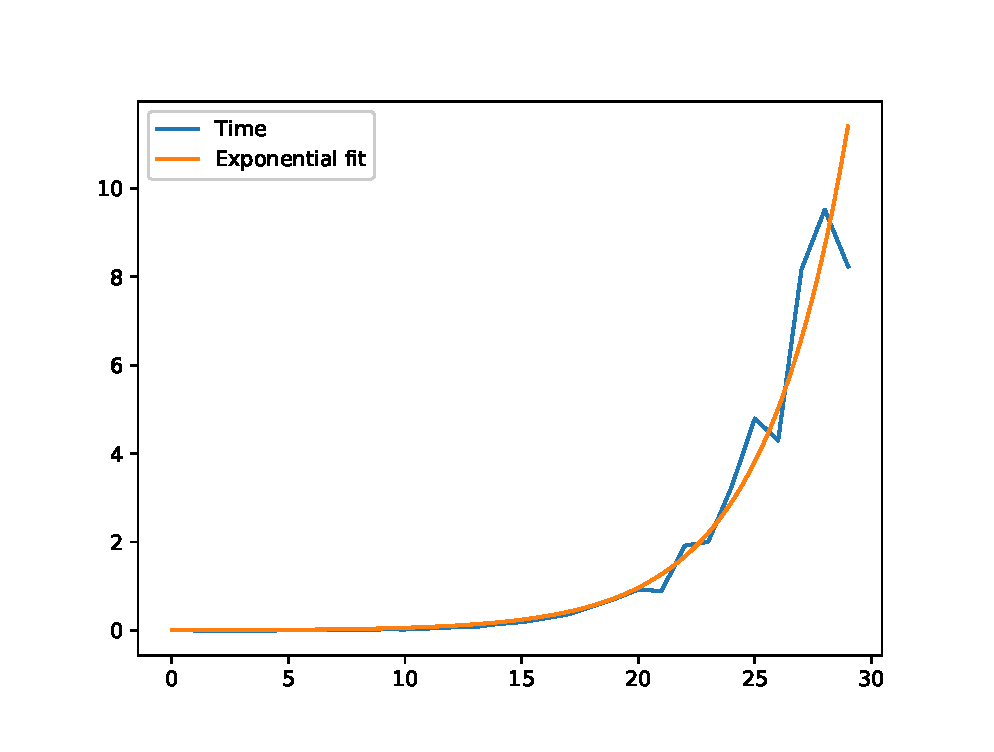
\includegraphics[width=0.9\textwidth]{time_graph}
    \caption{Tiempo de ejecución en relación al tamaño del problema}
    \label{fig:time_graph}
\end{figure}

Como se puede observar en la figura \ref{fig:time_graph}, el tiempo que tarda en
resolver el problema \texttt{Metric-FF} es exponencial respecto al tamaño de la
entrada (en este caso, el número de tareas).

\subsection{Ponderación extensión 4}

Se han probado varias ponderaciones entre el número de programadores y el tiempo total, en un caso con 6 tareas y 10 programadores. Se obtienen los siguientes resultados, según el peso del número de programadores:

\begin{table}[h]
\begin{longtable}{lll}
\toprule
Peso & Nº Programadores & Tiempo de ejecucion (s) \\
\midrule
\endhead
0 & 6 & 1.1 \\
0.8 & 6 & 1.0 \\
0.85 & 6 & 1.1 \\
0.9 & 5 & 13.58 \\
0.95 & 5 & 126.7 \\
\bottomrule
\end{longtable}
\end{table}

Por lo que observamos que la ponderación solo tiene resultados distintos a los de la extensión 3 si la ponderación del número de programadores es alta. Además, vemos que una ponderación excesivamente alta aumenta mucho el tiempo de ejecución, por lo que la dejamos en 0.9 para el número de programadores y 0.1 para el tiempo total.

\section{Problemas de prueba}

Para diseñar los juego de pruebas hemos usado un diseño incremental siguiendo el guión del enunciado de la práctica, es decir, hemos ido ampliando lentamente el problema según cada extensión, añadiendo los elementos que este necesita. Además hemos escogido 3 casos bases donde la cantidad de programadores y tarea se ha incrementado para poder obtener una visión más clara de los resultados obtenidos.

\subsection{Básico}

\subsubsection*{Conjunto 1}

INPUT:
\begin{lstlisting}[language=PDDL]
(define (problem test-01) (:domain planif)
    (:objects p1 p2 p3 p4 - Programador t1 t2 t3 - Tarea)
    (:init
        (= (habilidad p1) 1)
        (= (habilidad p2) 1)
        (= (habilidad p3) 3)
        (= (habilidad p4) 3) 

        (= (dificultad t1) 1)
        (= (dificultad t2) 2)
        (= (dificultad t3) 3)        
    )

    (:goal (forall (?t - Tarea) (realizada ?t)))
)
\end{lstlisting}

OUTPUT:
\begin{lstlisting}
step    0: REALIZAR P4 T3
        1: REALIZAR P4 T2
        2: REALIZAR P4 T1
\end{lstlisting}

\subsubsection*{Conjunto 2}

INPUT:
\begin{lstlisting}[language=PDDL]
(define (problem test) (:domain planif)
	(:objects p0 p1 p2 p3 p4 p5 p6 p7 p8 - Programador t0 t1 t2 t3 t4 - Tarea)
	(:init
		(= (habilidad p0) 1)
		(= (habilidad p1) 3)
		(= (habilidad p2) 3)
		(= (habilidad p3) 1)
		(= (habilidad p4) 1)
		(= (habilidad p5) 3)
		(= (habilidad p6) 1)
		(= (habilidad p7) 3)
		(= (habilidad p8) 3)
		
		(= (dificultad t0) 3)
		(= (dificultad t1) 3)
		(= (dificultad t2) 1)
		(= (dificultad t3) 3)
		(= (dificultad t4) 3)
		
	)
	(:goal
		(forall (?t - Tarea) (realizada ?t))
	)
)
\end{lstlisting}

OUTPUT:
\begin{lstlisting}
step    0: REALIZAR P8 T4
        1: REALIZAR P8 T3
        2: REALIZAR P8 T2
        3: REALIZAR P8 T1
        4: REALIZAR P8 T0
\end{lstlisting}

\subsubsection*{Conjunto 3}
INPUT:
\begin{lstlisting}[language=PDDL]
(define (problem test) (:domain planif)
	(:objects p0 p1 p2 p3 p4 p5 p6 p7 p8 p9 p10 p11 p12 - Programador t0 t1 t2 t3 t4 t5 t6 - Tarea)
	(:init
		(= (habilidad p0) 1)
		(= (habilidad p1) 1)
		(= (habilidad p2) 1)
		(= (habilidad p3) 2)
		(= (habilidad p4) 1)
		(= (habilidad p5) 2)
		(= (habilidad p6) 3)
		(= (habilidad p7) 3)
		(= (habilidad p8) 1)
		(= (habilidad p9) 2)
		(= (habilidad p10) 1)
		(= (habilidad p11) 1)
		(= (habilidad p12) 3)
		
		(= (dificultad t0) 3)
		(= (dificultad t1) 3)
		(= (dificultad t2) 3)
		(= (dificultad t3) 3)
		(= (dificultad t4) 1)
		(= (dificultad t5) 2)
		(= (dificultad t6) 3)
		
	)
	(:goal (forall (?t - Tarea) (realizada ?t))
	)
)
\end{lstlisting}

OUTPUT:
\begin{lstlisting}
step    0: REALIZAR P12 T6
        1: REALIZAR P12 T5
        2: REALIZAR P12 T4
        3: REALIZAR P12 T3
        4: REALIZAR P12 T2
        5: REALIZAR P12 T1
        6: REALIZAR P12 T0
\end{lstlisting}

\subsubsection{Conclusión}
El objetivo de este dominio es básicamente ver que todas las tareas son asociadas a un programador y que, además, lo hace correctamente respecto la habilidad de los programadores y la dificultad de la tarea. Podemos ver como la planificació se hace correctamente ya que en todos los casos escoge el último programador que tienen habilidad 3 y hace todas las tareas por lo tanto cumple con los requisitos básicos.

\subsection{Extensión 1}

\subsubsection*{Conjunto 1}

INPUT:
\begin{lstlisting}[language=PDDL]
(define (problem test-01) (:domain planif)
    (:objects p1 p2 p3 p4 - Programador t1 t2 t3 - Tarea)
    (:init
        (= (habilidad p1) 1)
        (= (habilidad p2) 1)
        (= (habilidad p3) 3)
        (= (habilidad p4) 3)
        
        (= (dificultad t1) 1)
        (= (dificultad t2) 2)
        (= (dificultad t3) 3)
        
    )

    (:goal (and
                (forall (?t - Tarea) (realizada ?t))
                (forall (?t - Tarea) (revisada ?t))
            )
    )
)
\end{lstlisting}

OUTPUT:
\begin{lstlisting}
step    0: REALIZAR P3 T3
        1: REVISAR P4 T3
        2: REALIZAR P1 T2
        3: REVISAR P4 T2
        4: REALIZAR P1 T1
        5: REVISAR P4 T1
\end{lstlisting}

\subsubsection*{Conjunto 2}
INPUT:
\begin{lstlisting}[language=PDDL]
(define (problem test) (:domain planif)
	(:objects p0 p1 p2 p3 p4 p5 p6 p7 p8 - Programador t0 t1 t2 t3 t4 - Tarea)
	(:init
		(= (habilidad p0) 1)
		(= (habilidad p1) 3)
		(= (habilidad p2) 3)
		(= (habilidad p3) 1)
		(= (habilidad p4) 1)
		(= (habilidad p5) 3)
		(= (habilidad p6) 1)
		(= (habilidad p7) 3)
		(= (habilidad p8) 3)
		
		(= (dificultad t0) 3)
		(= (dificultad t1) 3)
		(= (dificultad t2) 1)
		(= (dificultad t3) 3)
		(= (dificultad t4) 3)
		
	)
	(:goal (and
		(forall (?t - Tarea) (realizada ?t))
		(forall (?t - Tarea) (revisada ?t))
		)
	)
)
\end{lstlisting}

OUTPUT:
\begin{lstlisting}
step    0: REALIZAR P1 T4
        1: REVISAR P8 T4
        2: REALIZAR P1 T3
        3: REVISAR P8 T3
        4: REALIZAR P0 T2
        5: REVISAR P8 T2
        6: REALIZAR P1 T1
        7: REVISAR P8 T1
        8: REALIZAR P1 T0
        9: REVISAR P8 T0
\end{lstlisting}

\subsubsection*{Conjunto 3}
INPUT:
\begin{lstlisting}[language=PDDL]
(define (problem test) (:domain planif)
	(:objects p0 p1 p2 p3 p4 p5 p6 p7 p8 p9 p10 p11 p12 - Programador t0 t1 t2 t3 t4 t5 t6 - Tarea)
	(:init
		(= (habilidad p0) 1)
		(= (habilidad p1) 1)
		(= (habilidad p2) 1)
		(= (habilidad p3) 2)
		(= (habilidad p4) 1)
		(= (habilidad p5) 2)
		(= (habilidad p6) 3)
		(= (habilidad p7) 3)
		(= (habilidad p8) 1)
		(= (habilidad p9) 2)
		(= (habilidad p10) 1)
		(= (habilidad p11) 1)
		(= (habilidad p12) 3)
		
		(= (dificultad t0) 3)
		(= (dificultad t1) 3)
		(= (dificultad t2) 3)
		(= (dificultad t3) 3)
		(= (dificultad t4) 1)
		(= (dificultad t5) 2)
		(= (dificultad t6) 3)

		(= (total) 0)
	)
	(:goal (and
		(forall (?t - Tarea) (realizada ?t))
		(forall (?t - Tarea) (revisada ?t))
		)
	)
	(:metric minimize (total))
)
\end{lstlisting}

OUTPUT:
\begin{lstlisting}
step    0: REALIZAR P3 T6
        1: REVISAR P12 T6
        2: REALIZAR P0 T5
        3: REVISAR P12 T5
        4: REALIZAR P0 T4
        5: REVISAR P12 T4
        6: REALIZAR P3 T3
        7: REVISAR P12 T3
        8: REALIZAR P3 T2
        9: REVISAR P12 T2
       10: REALIZAR P3 T1
       11: REVISAR P12 T1
       12: REALIZAR P3 T0
       13: REVISAR P12 T0
\end{lstlisting}

\subsubsection{Conclusión}

La intención de este juego de pruebas es ver que funciona correctamente la acción de revisar, es decir que el programador que revisa la tarea $i$ no sea el mismo programador que haya realizado la tarea. En general vemos que escoge un programador para hacer todas las tareas de revisión y usa los demás para realizar las tareas, por ende, cumple con la condición de que el programador que realiza la tarea no es quien la revisa, además vemos que el programador escogido para hacer la revisión tiene habilidad 3 pues también se ajusta a la condición de revisión de cualquier tarea.

\subsection{Extensión 2}

\subsubsection*{Conjunto 1:}

INPUT:
\begin{lstlisting}[language=PDDL]
(define (problem test-01) (:domain planif)
    (:objects p1 p2 p3 p4 - Programador t1 t2 t3 - Tarea)
    (:init
        (= (habilidad p1) 1)
        (= (habilidad p2) 1)
        (= (habilidad p3) 3)
        (= (habilidad p4) 3)
        
        (= (calidad p1) 1)
        (= (calidad p2) 1)
        (= (calidad p3) 2)
        (= (calidad p4) 1)
        
        (= (dificultad t1) 1)
        (= (dificultad t2) 2)
        (= (dificultad t3) 3)
        
        (= (horas t1) 1)
        (= (horas t2) 2)
        (= (horas t3) 3)

        (= (total) 0)
    )
    (:goal (and
                (forall (?t - Tarea) (realizada ?t))
                (forall (?t - Tarea) (revisada ?t))
            )
    )
    (:metric minimize (total))
)
\end{lstlisting}

OUTPUT:
\begin{lstlisting}
step    0: REALIZAR P4 T3
        1: REALIZAR P4 T2
        2: REALIZAR P1 T1
        3: REVISAR P4 T1
        4: REVISAR P3 T2
        5: REVISAR P3 T3
\end{lstlisting}

\subsubsection*{Conjunto 2}
INPUT:
\begin{lstlisting}[language=PDDL]
(define (problem test) (:domain planif)
	(:objects p0 p1 p2 p3 p4 p5 p6 p7 p8 - Programador t0 t1 t2 t3 t4 - Tarea)
	(:init
		(= (habilidad p0) 1)
		(= (habilidad p1) 3)
		(= (habilidad p2) 3)
		(= (habilidad p3) 1)
		(= (habilidad p4) 1)
		(= (habilidad p5) 3)
		(= (habilidad p6) 1)
		(= (habilidad p7) 3)
		(= (habilidad p8) 3)
		
		(= (calidad p0) 2)
		(= (calidad p1) 1)
		(= (calidad p2) 1)
		(= (calidad p3) 1)
		(= (calidad p4) 2)
		(= (calidad p5) 2)
		(= (calidad p6) 1)
		(= (calidad p7) 2)
		(= (calidad p8) 2)
		
		(= (dificultad t0) 3)
		(= (dificultad t1) 3)
		(= (dificultad t2) 1)
		(= (dificultad t3) 3)
		(= (dificultad t4) 3)
		
		(= (horas t0) 11)
		(= (horas t1) 14)
		(= (horas t2) 10)
		(= (horas t3) 10)
		(= (horas t4) 13)
		
		(= (total) 0)
	)
	(:goal (and
		(forall (?t - Tarea) (realizada ?t))
		(forall (?t - Tarea) (revisada ?t))
		)
	)
	(:metric minimize (total))
)
\end{lstlisting}

OUTPUT:
\begin{lstlisting}
step    0: REALIZAR P1 T1
        1: REALIZAR P1 T4
        2: REALIZAR P1 T0
        3: REALIZAR P1 T3
        4: REALIZAR P1 T2
        5: REVISAR P8 T2
        6: REVISAR P8 T3
        7: REVISAR P8 T0
        8: REVISAR P8 T4
        9: REVISAR P8 T1
\end{lstlisting}

\subsubsection*{Conjunto 3}
INPUT:
\begin{lstlisting}[language=PDDL]
(define (problem test) (:domain planif)
	(:objects p0 p1 p2 p3 p4 p5 p6 p7 p8 p9 p10 p11 p12 - Programador t0 t1 t2 t3 t4 t5 t6 - Tarea)
	(:init
		(= (habilidad p0) 1)
		(= (habilidad p1) 1)
		(= (habilidad p2) 1)
		(= (habilidad p3) 2)
		(= (habilidad p4) 1)
		(= (habilidad p5) 2)
		(= (habilidad p6) 3)
		(= (habilidad p7) 3)
		(= (habilidad p8) 1)
		(= (habilidad p9) 2)
		(= (habilidad p10) 1)
		(= (habilidad p11) 1)
		(= (habilidad p12) 3)
		
		(= (calidad p0) 1)
		(= (calidad p1) 1)
		(= (calidad p2) 1)
		(= (calidad p3) 2)
		(= (calidad p4) 1)
		(= (calidad p5) 1)
		(= (calidad p6) 2)
		(= (calidad p7) 2)
		(= (calidad p8) 2)
		(= (calidad p9) 1)
		(= (calidad p10) 1)
		(= (calidad p11) 2)
		(= (calidad p12) 1)
		
		(= (dificultad t0) 3)
		(= (dificultad t1) 3)
		(= (dificultad t2) 3)
		(= (dificultad t3) 3)
		(= (dificultad t4) 1)
		(= (dificultad t5) 2)
		(= (dificultad t6) 3)
		
		(= (horas t0) 10)
		(= (horas t1) 5)
		(= (horas t2) 11)
		(= (horas t3) 9)
		(= (horas t4) 6)
		(= (horas t5) 6)
		(= (horas t6) 4)
		
		(= (total) 0)
	)
	(:goal (and
		(forall (?t - Tarea) (realizada ?t))
		(forall (?t - Tarea) (revisada ?t))
		)
	)
	(:metric minimize (total))
)
\end{lstlisting}

OUTPUT:
\begin{lstlisting}
step    0: REALIZAR P12 T2
        1: REALIZAR P12 T0
        2: REALIZAR P12 T3
        3: REALIZAR P5 T5
        4: REALIZAR P0 T4
        5: REALIZAR P12 T1
        6: REALIZAR P12 T6
        7: REVISAR P9 T6
        8: REVISAR P9 T1
        9: REVISAR P12 T4
       10: REVISAR P12 T5
       11: REVISAR P9 T3
       12: REVISAR P9 T0
       13: REVISAR P9 T2
\end{lstlisting}

\subsubsection{Conclusión}

En estos casos de prueba queremos ver que la planificació minimiza correctamente el tiempo total para hacer las tareas, es decir realizarlo y revisarlo. Como podemos ver en el conjunto 3 respecto en la extensión anterior, P3 deja de realizar las tareas y se sustituye por otro programadores, eso es debido a que P3 realiza los trabajos con calidad 2 y, por lo tanto, genera una tarea adicional de 2 horas y, claramente, no será óptimo. En los demás conjuntos también se puede observar como los programadores que realizan las tareas son aquellos que tienen calidad 1 y no 2.

\subsection{Extensión 3}

\subsubsection*{Conjunto 1}
INPUT:
\begin{lstlisting}[language=PDDL]
(define (problem test-01) (:domain planif)
    (:objects p1 p2 p3 p4 - Programador t1 t2 t3 - Tarea)
    (:init
        (= (habilidad p1) 1)
        (= (habilidad p2) 1)
        (= (habilidad p3) 3)
        (= (habilidad p4) 3)
        
        (= (calidad p1) 1)
        (= (calidad p2) 1)
        (= (calidad p3) 2)
        (= (calidad p4) 1)
        
        (= (dificultad t1) 1)
        (= (dificultad t2) 2)
        (= (dificultad t3) 3)
        
        (= (horas t1) 1)
        (= (horas t2) 2)
        (= (horas t3) 3)

        (= (tareas-realizadas p1) 0)
        (= (tareas-realizadas p2) 0)
        (= (tareas-realizadas p3) 0)
        (= (tareas-realizadas p4) 0)
        
        (= (total) 0)
    )
    (:goal (and
                (forall (?t - Tarea) (realizada ?t))
                (forall (?t - Tarea) (revisada ?t))
            )
    )
    (:metric minimize (total))
)
\end{lstlisting}

OUTPUT:
\begin{lstlisting}
step    0: REALIZAR P4 T3
        1: REALIZAR P3 T2
        2: REALIZAR P1 T1
        3: REVISAR P1 T2
        4: REVISAR P2 T1
        5: REVISAR P3 T3
\end{lstlisting}

\subsubsection*{Conjunto 2}

INPUT:
\begin{lstlisting}[language=PDDL]
(define (problem test) (:domain planif)
	(:objects p0 p1 p2 p3 p4 p5 p6 p7 p8 - Programador t0 t1 t2 t3 t4 - Tarea)
	(:init
		(= (habilidad p0) 1)
		(= (habilidad p1) 3)
		(= (habilidad p2) 3)
		(= (habilidad p3) 1)
		(= (habilidad p4) 1)
		(= (habilidad p5) 3)
		(= (habilidad p6) 1)
		(= (habilidad p7) 3)
		(= (habilidad p8) 3)
		
		(= (calidad p0) 2)
		(= (calidad p1) 1)
		(= (calidad p2) 1)
		(= (calidad p3) 1)
		(= (calidad p4) 2)
		(= (calidad p5) 2)
		(= (calidad p6) 1)
		(= (calidad p7) 2)
		(= (calidad p8) 2)
		
		(= (tareas-realizadas p0) 0)
		(= (tareas-realizadas p1) 0)
		(= (tareas-realizadas p2) 0)
		(= (tareas-realizadas p3) 0)
		(= (tareas-realizadas p4) 0)
		(= (tareas-realizadas p5) 0)
		(= (tareas-realizadas p6) 0)
		(= (tareas-realizadas p7) 0)
		(= (tareas-realizadas p8) 0)
		
		(= (dificultad t0) 3)
		(= (dificultad t1) 3)
		(= (dificultad t2) 1)
		(= (dificultad t3) 3)
		(= (dificultad t4) 3)
		
		(= (horas t0) 11)
		(= (horas t1) 14)
		(= (horas t2) 10)
		(= (horas t3) 10)
		(= (horas t4) 13)
		
		(= (total) 0)
	)
	(:goal (and
		(forall (?t - Tarea) (realizada ?t))
		(forall (?t - Tarea) (revisada ?t))
		)
	)
	(:metric minimize (total))
)
\end{lstlisting}

OUTPUT:
\begin{lstlisting}
step    0: REALIZAR P1 T1
        1: REALIZAR P1 T4
        2: REALIZAR P2 T0
        3: REALIZAR P2 T2
        4: REALIZAR P5 T3
        5: REVISAR P0 T2
        6: REVISAR P5 T0
        7: REVISAR P7 T1
        8: REVISAR P7 T3
        9: REVISAR P8 T4
\end{lstlisting}

\subsubsection*{Conjunto 3}
INPUT:
\begin{lstlisting}[language=PDDL]
(define (problem test) (:domain planif)
	(:objects p0 p1 p2 p3 p4 p5 p6 p7 p8 p9 p10 p11 p12 - Programador t0 t1 t2 t3 t4 t5 t6 - Tarea)
	(:init
		(= (habilidad p0) 1)
		(= (habilidad p1) 1)
		(= (habilidad p2) 1)
		(= (habilidad p3) 2)
		(= (habilidad p4) 1)
		(= (habilidad p5) 2)
		(= (habilidad p6) 3)
		(= (habilidad p7) 3)
		(= (habilidad p8) 1)
		(= (habilidad p9) 2)
		(= (habilidad p10) 1)
		(= (habilidad p11) 1)
		(= (habilidad p12) 3)
		
		(= (calidad p0) 1) %1
		(= (calidad p1) 1) %1
		(= (calidad p2) 1) %1
		(= (calidad p3) 2) %2
		(= (calidad p4) 1) %1
		(= (calidad p5) 1) %2
		(= (calidad p6) 2) %3
		(= (calidad p7) 2) %3
		(= (calidad p8) 2) %1
		(= (calidad p9) 1) %2
		(= (calidad p10) 1) %1
		(= (calidad p11) 2) %1
		(= (calidad p12) 1) %3
		
		(= (tareas-realizadas p0) 0)
		(= (tareas-realizadas p1) 0)
		(= (tareas-realizadas p2) 0)
		(= (tareas-realizadas p3) 0)
		(= (tareas-realizadas p4) 0)
		(= (tareas-realizadas p5) 0)
		(= (tareas-realizadas p6) 0)
		(= (tareas-realizadas p7) 0)
		(= (tareas-realizadas p8) 0)
		(= (tareas-realizadas p9) 0)
		(= (tareas-realizadas p10) 0)
		(= (tareas-realizadas p11) 0)
		(= (tareas-realizadas p12) 0)
		
		(= (dificultad t0) 3)
		(= (dificultad t1) 3)
		(= (dificultad t2) 3)
		(= (dificultad t3) 3)
		(= (dificultad t4) 1)
		(= (dificultad t5) 2)
		(= (dificultad t6) 3)
		
		(= (horas t0) 10)
		(= (horas t1) 5)
		(= (horas t2) 11)
		(= (horas t3) 9)
		(= (horas t4) 6)
		(= (horas t5) 6)
		(= (horas t6) 4)

		(= (total) 0)
	)
	(:goal (and
		(forall (?t - Tarea) (realizada ?t))
		(forall (?t - Tarea) (revisada ?t))
		)
	)
	(:metric minimize (total))
)
\end{lstlisting}

OUTPUT:
\begin{lstlisting}
step    0: REALIZAR P12 T2
        1: REALIZAR P6 T0
        2: REALIZAR P6 T3
        3: REALIZAR P0 T4
        4: REALIZAR P5 T5
        5: REALIZAR P7 T1
        6: REALIZAR P12 T6
        7: REVISAR P0 T5
        8: REVISAR P1 T4
        9: REVISAR P3 T0
       10: REVISAR P3 T1
       11: REVISAR P5 T2
       12: REVISAR P7 T3
       13: REVISAR P9 T6

\end{lstlisting}

\subsubsection{Conclusión}

La intención de estos juegos de pruebas es ver como cada programador solo realiza dos tareas, además queremos resaltar la propiedad de la extensión 2, es decir, no solo queremos planificar solo dos tareas para cada programador sinó que escoge aquellos con calidad 1 para realizar las tareas. En el conjunto 1 vemos que hay una excepción y es P3, esto no pasaba en la extensión 2 debido a que P4 podía realizar más de 2 tareas, en este caso es más rentable hacer dos horas de revisión que las dos horas adicionales que tendría que gastar un programador con habilidad menor. Con el conjunto 2 pasa exactamente lo mismo, se prefiere que P5 haga la tarea en vez de que lo haga otro de habilidad menor. En el conjunto 3 és un poco más exagerado, pero es debido a que la cantidad de programadores con habilidad 3 es bastante reducido y la mayoría de las tareas tienen dificultad 3, por ende, solo puede asignarlos a programadores con calidad 2. Además la planificación también cumple con la condición de que cada programador solo puede tener asignada a una tarea.

\subsection{Extensión 4}

\subsubsection*{Conjunto 1}

INPUT:
\begin{lstlisting}[language=PDDL]
(define (problem test-01) (:domain planif)
    (:objects p1 p2 p3 p4 - Programador t1 t2 t3 - Tarea)
    (:init
        (= (habilidad p1) 1)
        (= (habilidad p2) 1)
        (= (habilidad p3) 3)
        (= (habilidad p4) 3)
        
        (= (calidad p1) 1)
        (= (calidad p2) 1)
        (= (calidad p3) 2)
        (= (calidad p4) 1)
        
        (= (dificultad t1) 1)
        (= (dificultad t2) 2)
        (= (dificultad t3) 3)
        
        (= (horas t1) 1)
        (= (horas t2) 2)
        (= (horas t3) 3)

        (= (tareas-realizadas p1) 0)
        (= (tareas-realizadas p2) 0)
        (= (tareas-realizadas p3) 0)
        (= (tareas-realizadas p4) 0)
        
        (= (total) 0)
        (= (num-personas) 0)
    )
    (:goal (and
                (forall (?t - Tarea) (realizada ?t))
                (forall (?t - Tarea) (revisada ?t))
            )
    )
    (:metric minimize(+ (* (num-personas) 0.5) (* (total) 0.5)))
)
\end{lstlisting}

OUTPUT:
\begin{lstlisting}
step    0: REALIZAR P4 T3
        1: REALIZAR P3 T2
        2: REALIZAR P4 T1
        3: REVISAR P3 T3
        4: REVISAR P1 T1
        5: REVISAR P1 T2
\end{lstlisting}

\subsubsection*{Conjunto 2}

INPUT:
\begin{lstlisting}[language=PDDL]
(define (problem test) (:domain planif)
	(:objects p0 p1 p2 p3 p4 p5 p6 p7 p8 - Programador t0 t1 t2 t3 t4 - Tarea)
	(:init
		(= (habilidad p0) 1)
		(= (habilidad p1) 3)
		(= (habilidad p2) 3)
		(= (habilidad p3) 1)
		(= (habilidad p4) 1)
		(= (habilidad p5) 3)
		(= (habilidad p6) 1)
		(= (habilidad p7) 3)
		(= (habilidad p8) 3)
		
		(= (calidad p0) 2)
		(= (calidad p1) 1)
		(= (calidad p2) 1)
		(= (calidad p3) 1)
		(= (calidad p4) 2)
		(= (calidad p5) 2)
		(= (calidad p6) 1)
		(= (calidad p7) 2)
		(= (calidad p8) 2)
		
		(= (tareas-realizadas p0) 0)
		(= (tareas-realizadas p1) 0)
		(= (tareas-realizadas p2) 0)
		(= (tareas-realizadas p3) 0)
		(= (tareas-realizadas p4) 0)
		(= (tareas-realizadas p5) 0)
		(= (tareas-realizadas p6) 0)
		(= (tareas-realizadas p7) 0)
		(= (tareas-realizadas p8) 0)
		
		(= (dificultad t0) 3)
		(= (dificultad t1) 3)
		(= (dificultad t2) 1)
		(= (dificultad t3) 3)
		(= (dificultad t4) 3)
		
		(= (horas t0) 11)
		(= (horas t1) 14)
		(= (horas t2) 10)
		(= (horas t3) 10)
		(= (horas t4) 13)
		
		(= (total) 0)
		(= (num-personas) 0)
	)
	(:goal (and
		(forall (?t - Tarea) (realizada ?t))
		(forall (?t - Tarea) (revisada ?t))
		)
	)
	(:metric minimize (+ (* (num-personas) 0.5) (* (total) 0.5)))
)
\end{lstlisting}

OUTPUT:
\begin{lstlisting}
step    0: REALIZAR P1 T1
        1: REALIZAR P1 T4
        2: REALIZAR P2 T0
        3: REALIZAR P2 T2
        4: REALIZAR P5 T3
        5: REVISAR P8 T2
        6: REVISAR P8 T3
        7: REVISAR P7 T4
        8: REVISAR P7 T0
        9: REVISAR P5 T1
\end{lstlisting}

\subsubsection*{Conjunto 3}
INPUT:
\begin{lstlisting}[language=PDDL]
(define (problem test) (:domain planif)
	(:objects p0 p1 p2 p3 p4 p5 p6 p7 p8 p9 p10 p11 p12 - Programador t0 t1 t2 t3 t4 t5 t6 - Tarea)
	(:init
		(= (habilidad p0) 1)
		(= (habilidad p1) 1)
		(= (habilidad p2) 1)
		(= (habilidad p3) 2)
		(= (habilidad p4) 1)
		(= (habilidad p5) 2)
		(= (habilidad p6) 3)
		(= (habilidad p7) 3)
		(= (habilidad p8) 1)
		(= (habilidad p9) 2)
		(= (habilidad p10) 1)
		(= (habilidad p11) 1)
		(= (habilidad p12) 3)
		
		(= (calidad p0) 1)
		(= (calidad p1) 1)
		(= (calidad p2) 1)
		(= (calidad p3) 2)
		(= (calidad p4) 1)
		(= (calidad p5) 1)
		(= (calidad p6) 2)
		(= (calidad p7) 2)
		(= (calidad p8) 2)
		(= (calidad p9) 1)
		(= (calidad p10) 1)
		(= (calidad p11) 2)
		(= (calidad p12) 1)
		
		(= (tareas-realizadas p0) 0)
		(= (tareas-realizadas p1) 0)
		(= (tareas-realizadas p2) 0)
		(= (tareas-realizadas p3) 0)
		(= (tareas-realizadas p4) 0)
		(= (tareas-realizadas p5) 0)
		(= (tareas-realizadas p6) 0)
		(= (tareas-realizadas p7) 0)
		(= (tareas-realizadas p8) 0)
		(= (tareas-realizadas p9) 0)
		(= (tareas-realizadas p10) 0)
		(= (tareas-realizadas p11) 0)
		(= (tareas-realizadas p12) 0)
		
		(= (dificultad t0) 3)
		(= (dificultad t1) 3)
		(= (dificultad t2) 3)
		(= (dificultad t3) 3)
		(= (dificultad t4) 1)
		(= (dificultad t5) 2)
		(= (dificultad t6) 3)
		
		(= (horas t0) 10)
		(= (horas t1) 5)
		(= (horas t2) 11)
		(= (horas t3) 9)
		(= (horas t4) 6)
		(= (horas t5) 6)
		(= (horas t6) 4)
		
		(= (total) 0)
		(= (num-personas) 0)
	)
	(:goal (and
		(forall (?t - Tarea) (realizada ?t))
		(forall (?t - Tarea) (revisada ?t))
		)
	)
	(:metric minimize (+ (* (num-personas) 0.5) (* (total) 0.5)))
)
\end{lstlisting}

OUTPUT:
\begin{lstlisting}
step    0: REALIZAR P12 T2
        1: REALIZAR P6 T0
        2: REALIZAR P6 T3
        3: REALIZAR P0 T4
        4: REALIZAR P5 T5
        5: REALIZAR P5 T1
        6: REALIZAR P12 T6
        7: REVISAR P7 T2
        8: REVISAR P7 T3
        9: REVISAR P3 T6
       10: REVISAR P3 T0
       11: REVISAR P0 T5
       12: REVISAR P9 T1
       13: REVISAR P9 T4
\end{lstlisting}

\subsubsection{Conclusión}

Por último, queremos ver que nuestra métrica funciona correctamente con los juegos de pruebas de la extensión 2. En general queremos ver que la planificació no solo minimiza el tiempo sinó también la cantidad de programadores realizando alguna tarea. En el conjunto 1 que es el más reducido podemos ver en comparación a la extensión anterior que solo utiliza 3 programadores en vez de 4, por lo tanto se consigue lo pedido. En los conjuntos 2 y 3 también se puede ver que se ha reducido en uno la cantidad de programadores trabajando. Por lo tanto se logra los objetivos establecidos.

\end{document}

